\chapter{The Atoms} \label{ChapterAboutTheAtoms}
\section{Overview of relevant atomic transitions}

The system is designed to stimulate Raman transitions between the hyperfine $^2$S$_{1/2}$ ($5s$) ground states corresponding to $F=4$ and $F=5$. The intermediate state is the $^2$P$_{3/2}$ ($5p$) state. 

\begin{figure}
\centerline{
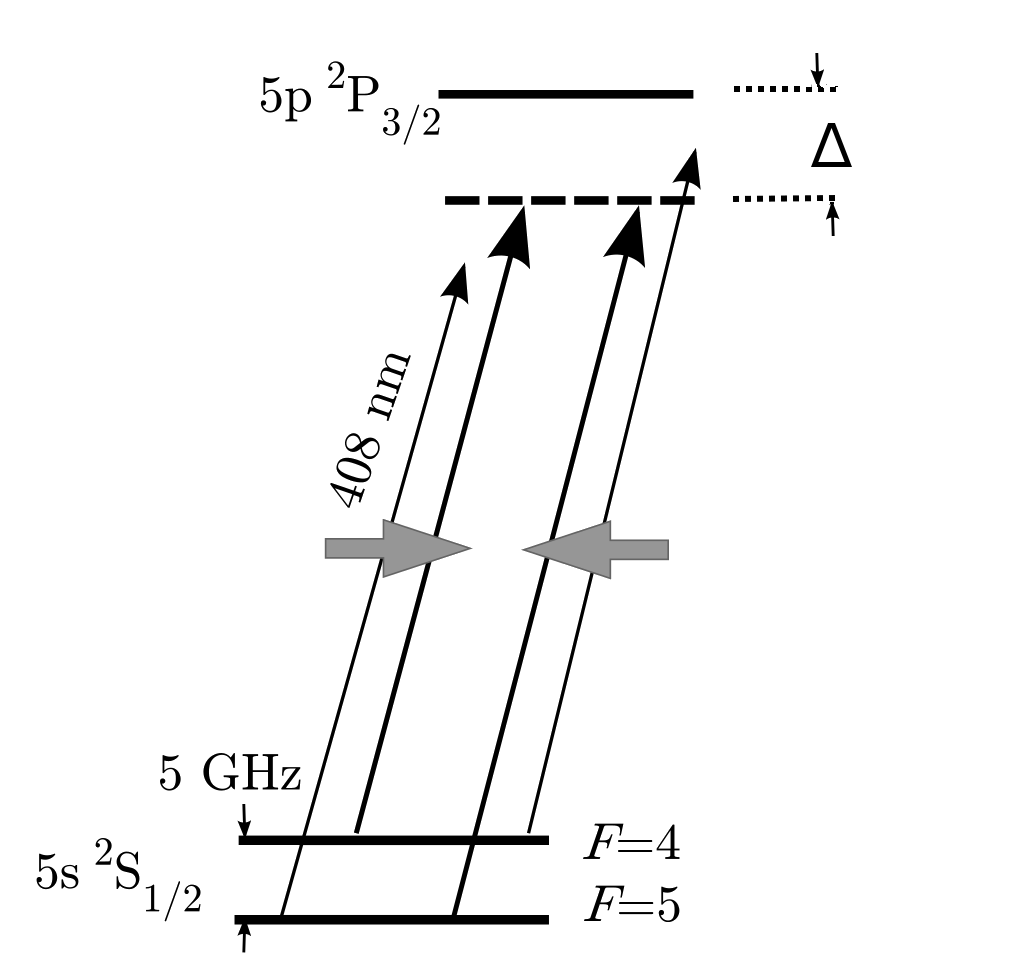
\includegraphics[totalheight=0.3\textheight]{E_level_from_proposal}
}
\caption[Energy Level Diagram for $^{87}$Sr+]{Energy Level Diagram for $^{87}$Sr+. The hyperfine ground states are separated by a small energy. Diagram is not to scale: a scaled diagram would show the splitting between the $F=4$ and $F=5$ states to be about 147,000 times smaller than the splitting between the $^2$S$_{1/2}$ states and the $^2$P$_{3/2}$ states.}
\end{figure}

Our objective is to calculate the necessary intensity and beam waist that will allow our lasers to impart the $\pi$ and $\pi/2$ pulses to the atoms as they make their way through the chamber. 

In order to do this, we first review the various relevant states of this atom and the quantum numbers used to describe them. Then we move onto a discussion of some of the basic aspects of hyperfine structure. We will then model the atom as a three state system and obtain an expression relating the magnitude and frequency of the electric field to the Rabi frequencies of our two transitions. Finally, we calculate the total transition rate for the 3 state system and we tabulate the beam parameters that will produce the requisite electric field strengths for the correct amounts of time to produce the transition.

The discussion that follows is strictly geared towards


In Ref.\ \cite{cjeDiss}, this calculation is performed, but some of the details are left mysterious. In particular, no source is cited for any of the physical parameters of the $^{87}$Sr+ atom (e.g. the dipole moment values, the transition width, the saturation parameter). We hope to reproduce this calculation with more details.  

\section{States and Quantum Numbers}

We model the Hamiltonian of the Strontium ions by analogy to the Hamiltonian of a single-electron atom. 
In a single electron atom, the solution to the Schr\"odinger equation describing the electron is solved by separation of variables.
 Each solution is a product of a spherically symmetric function that depends only on the distance $r$ from the nucleus and the spherical harmonics.
This is because the orbital angular momentum operator $\mathbf{L}$ commutes with such a Hamiltonian. In fact, the orbital angular momentum operator commutes with any Hamiltonian with a spherically symmetric potential.
Thus, the eigenstates of any spherically symmetrical Hamiltonian can be treated precisely as they are in a one-electron case. 

In the case of $^{87}$Sr+, there is only one electron in the valence band. The inner shells are full and we assume that the symmetry is such that the eigenstates of the atom will also be eigenstates of the orbital angular momentum operator, $\mathbf{L}$.
 The system also involves two other angular momentum operators: the spin operator for the valence electron, $\mathbf{S}$\footnote{The spin of the electrons on the inner shells cancels and adds to 0} and the spin of the nucleus $\mathbf{I}$.
\footnote{Here and throughout, we will generally use the boldface $\mathbf{I}$ to mean the operator while the unbolded $I$ will mean the eigenvalue, though for the most part, context will be the most reliable way to distinguish between the two.}
We will first approximate the Hamiltonian by assuming that there is no coupling that is dependent on the spin. 
The hyperfine interaction will be modeled as a perturbation on top of this.

The ``good'' quantum numbers for describing the internal states of a $^{87}$Sr+ ion are $F$,$J$,$L$,$S$,$m_f$ and $n$\cite{experimental_hyperfine_alkali_arimondo}\cite{cuaMITnotes} where $F$,$J$,$L$,$S$,$m_f$ take on their usual meanings (see \ref{quantumNumberQuickref})

\begin{table}[h!]
\centering
\begin{tabular}{|c|l|}
\hline
Quantum Number & Definition and comment \\ \hline \hline
L & Orbital angular momentum of valence electron. \\ \hline
S & Spin of valence electron. Takes on values $\pm 1/2$ \\ \hline
I & Nuclear spin. For $^{87}$Sr$^+$, $I=9/2$ \\ \hline
J & Total valence electron angular momentum. $\mathbf{J}=\mathbf{L}+\mathbf{S}$ \\ \hline
F & Total angular momentum $\mathbf{F}=\mathbf{I}+\mathbf{J}$ \\ \hline
$m_f$ & Eigenvalue of $\mathbf{F}_z$.\\ \hline
\end{tabular}
\caption{The quantum numbers used to describe the internal state of the $^{87}$Sr+ ion. These are conventional choices, the table is only for the reader's convenience.}
\label{quantumNumberQuickref}
\end{table}

The Hamiltonian has the form 

\begin{equation}
H_0=\sum |F,J,L,S,M_f,n\rangle E \langle F,J,L,S,M_f,n|
\end{equation}
We neglect all except the following states: %why does the ground state J not play into it at all?
%I just realized I have no idea where to find the information on the hyperfine splitting of the Sr+ 
%also, IDK what to do about the the Nuclear spin numbers of the upper state. 
%I have this http://link.springer.com/article/10.1007%2FBF00568145

\begin{table}[h]
\centering
\begin{tabular}{|l|l|||r|}
\hline
$F=4$ $^2$S$_{1/2} (5s)$ & Ground state  \\ \hline
$F=5$ $^2$S$_{1/2} (5s)$ & Ground state  \\ \hline
$F=3$ $^2$P$_{3/2} (5p)$ & Intermediate state  \\ \hline
$F=4$ $^2$P$_{3/2} (5p)$ & Intermediate state  \\ \hline
$F=5$ $^2$P$_{3/2} (5p)$ & Intermediate state  \\ \hline
$F=6$ $^2$P$_{3/2} (5p)$ & Intermediate state  \\ \hline
\end{tabular}
\caption{Relevant states}
\label{tableOfStates}
\end{table}

\section{Review of Hyperfine Splitting}

The hyperfine splitting arises from interactions between the nucleus and the electrons. In general, we can split out the Hamiltonian of the Hyperfine interaction as follows: 

\begin{equation}
H=H_0+H_{\mathrm{hfs}}
\end{equation}

where $H$ represents the total Hamiltonian of the system, $H_0$ represents the Hamiltonian neglecting the hyperfine interaction and $H_{\mathrm{hfs}}$ represents the piece of the Hamiltonian that takes the hyperfine interaction into account. 

The standard expansion of $H_{\mathrm{hfs}}$ in the literature is:  

\begin{equation}
H_{\mathrm{hfs}}=\sum_k \mathbf{T}^{(k)} \cdot \mathbf{M}^{(k)} \label{hfs_hamiltonian_eqn}
\end{equation}
\cite{schwartz_hyperfine_expansion}
\cite{experimental_hyperfine_alkali_arimondo}
\cite{chinesePhysics}
%\footnote{todo: cite that review article and the lecture notes you found}

where $\mathbf{T}^{(k)}$ and $\mathbf{M}^{(k)}$ are irreducible spherical tensor operators of rank $k$.
 $\mathbf{T}^{(k)}$ represents information about the electron.
The generator of its rotations is the electron total angular momentum, $\mathbf{J}$. %In other words, it satisfies the commutation relationship:

%\begin{equation}
%[\mathbf{J}_i,\mathbf{T}^{(k)}_q]=
%\end{equation}
%\footnote{I know this is in Sakurai, but I also looked at wikipedia.}

$\mathbf{M}^{(k)}$ represents the nucleus and the generator of its rotation group is the nuclear spin $\mathbf{I}$.\cite{experimental_hyperfine_alkali_arimondo}\cite{schwartz_hyperfine_expansion}
\cite{sobelman_spectra}
%\footnote{In fact, \cite{schwartz_hyperfine_expansion} claims that it commutes with $\mathbf{J}$, but I don't believe this is possible. In order for it to be rotationally invariant, it must not commute with it}.

\footnote{Recall that the dot product for spherical tensors of arbitrary rank is defined as follows:
\begin{equation}
\mathbf{T}^{(k)}\cdot\mathbf{M}^{(k)}=\sum (-1)^qT_q^{(k)}M_{-q}^{(k)}
\end{equation}
}

The expansion of the hyperfine interaction in Eq.\ \ref{hfs_hamiltonian_eqn} encapsulates some important ideas.
Notice 
\footnote{must the perturbed states exist before? Can it split?} 
Eq.\ \ref{hfs_hamiltonian_eqn} shows explicitly how the operator transforms under rotations. Specifically, it shows that, by using these tensors, we could the coupling should remain the same under rotations.
Secondly, each term in the Hamiltonian represents coupling of a different electric or magnetic multipole moment. 

So, for example, 


It is interesting to note that the odd values of $k$ correspond to magnetic interactions while the even values correspond to electric interactions. That is to say that there is no electric dipole interaction between the electrons and the nucleus, but there is a magnetic dipole ($k=1$), while there is an electric quadrupole coupling, but no magnetic quadrupole, etc
\cite{experimental_hyperfine_alkali_arimondo}
.
The reason that the coupling can be described entirely in terms of scalar products of spherical tensors probably arises from the fact that the electronic wave function and the electric and magnetic fields created by the nucleus are centered around the same point. The electromagnetic fields created by the nucleus and the electronic wave function can both be expanded in terms of spherical harmonics. This can be seen in Ref.\ \cite{schwartz_hyperfine_expansion}. It can be seen that this more or less work in other, more ad-hoc discussions of hyperfine structure, like the one in Ref.\ \cite{cuaMITnotes}. 

In general, the most important contributions to the Hyperfine splitting come from the magnetic dipole contribution and the electric quadrupole contribution. 


\subsection{Hyperfine $A$ and $B$ coefficients}
There are various ways to estimate or calculate the hyperfine coefficients. However, for our purposes they are generally looked up and found by either experiment or numerical calculations. \cite{cuaMITnotes}. 


The magnetic dipole contribution to the Hyperfine splitting arises from coupling between the electron's total angular momentum and the 



\begin{equation}
E_{\mathrm{hfs}}=\frac{1}{2}AC+BC(C+1)
\end{equation}

where 

\begin{equation}
C=[F(F+1)-J(J+1)-I(I+1)]
\end{equation}

\footnote{this is from those MIT notes}

Ref.\ \cite{safronova2photon} gives and cites various values of the $A$ and $B$ coefficients. The ones relevant to our experiment are 

\begin{table}[h]
\centering
\begin{tabular}{|l|r|r|r|}
\hline
Level &  $A^{\mathrm{(SDpT)}}$ &$A^{\mathrm{(theor)}}$ & $A^{\mathrm{(expt)}}$ \\ \hline \hline
$5s ^2$S$_{1/2}$&-997.85 MHz& -1000 MHz& -1000.473673(11) MHz\\ \hline
$5p ^2$P$_{3/2}$&-35.26 MHz&-35.3 MHz&-36.0(04) MHz\\ \hline
\end{tabular}
\end{table}

\begin{table}[h]
\centering
\hline
Level &  $B^{\mathrm{(SDpT)}}$ &$B^{\mathrm{(theor)}}$ & $B^{\mathrm{(expt)}}$ \\ \hline \hline
$5s ^2$S$_{1/2}$&&0  MHz&  \\ \hline
$5p ^2$P$_{3/2}$&88.94MHz&271MHz$/b$$\times 0.327(24)$b$=88.68$MHz&88.5(54) \\ \hline
\end{tabular}
\end{table}


Now, to include the nuclear spin,$I$, we will use $F=J+I$. 

The Hamiltonian for a Hydrogen-like atom is: 

\begin{equation}
H=\frac{1}{2m}(\mathbf{p}-e\mathbf{A})^2+\phi(\mathbf{r})
\end{equation}

Normally, one takes this and then splits it into two Hamiltonians: 

\begin{equation}
H=H_0+V
\end{equation}
where 
\begin{equation}
H_0=\frac{\mathbf{p}^2}{2m}+\phi(\mathbf{r})
\end{equation}
and $V$ is written in terms of $\mathbf{A}$. They usually neglect the terms that are higher than second order in $\mathbf{A}$.

We proceed similarly. 

We assume that our Hamiltonian has the form 

\begin{equation}
H=H_0+V
\end{equation}


\footnote{Is there a static, external magnetic field? I seem to remember that there was.}



%the 0 -- when things from different vector spaces are their 0s, they make the other one 0. I mean, it's almost like 0 transcends its own vector space in the direct product. 

%OK, where does the energy plug in ? 

%OK, so I don't understand why it makes sense to take a $\mathbf{p}$ operator and use it on the $\mathbf{A}$ vector. Ah, well, $\mathbf{A}$ is an operator whose components interact with components of $\mathbf{r}$ in a regular way 
Oh, OK. So we are summing over all the z components of F?


$F$, we find that we must combine this with yet another 

Here, we have opted to look at the simultaneous eigenstates of the $F$,the The $^2$S states can be rewritten as a sum of eigenstates of the $\vec{J}$ and $\vec{F}$ operators. 


The Hamiltonian will be the sum of the original Hamiltonian 

First, we will write the complete Hamiltonian of the system.
Then, the new Hamiltonian, $H$, is given by 

\begin{equation}
H=H_0+V
\end{equation}
rotating wave approximation (RWA). Let $H_0$ be the Hamiltonian of our unperturbed system (the atom) and let $V$ be the perturbation (which we will use to model the electric field). 


Now, we can move to the interaction picture in the standard way. Let $|\alpha\rangle$ be the eigenstate of $H_0$, the unperturbed Hamiltonian: 

\begin{equation}
|\alpha\rangle_I=e^{-iE_\alpha t/h}|\alpha\rangle
\end{equation}

Then, 
%I don't know whether to use I or J. I mean, are there now tons of terms? 
\begin{align}
-i\hbar \frac{d}{dt}|n\rangle = 
\end{align}

\section{Finding the Dipole Moment Matrix Operator}
We would like to carefully determine the value of this. According to Ref.\ \cite{safronova2photon} the magnitude of the dipole moment operator is -4.35075 a. u. \footnote{atomic units, $a_0 e$} as calculated using the all-order, relativistic SD method. It is useful to compare this to the value obtained from at least one other source \footnote{I want to make sure the units and conventions are what I think they are.}. According to the NIST atomic spectra database, $A_{ki}=1.41e8$ s$^{-1}$ \cite{NISTasd}. This seems to be the Einstein A coefficient associated only with the decays from this state. If this is the case, then we use this equation from Ref.\ \cite{demilleBudkerKimball}:  
\begin{equation}
|\langle f ||d|| i \rangle|^2 = (4 \pi \epsilon_0) \frac{3 \hbar c^3}{4 \omega_0^3} (2 J'+1) A_{ki}\label{budkerAeqn} 
\end{equation}

This comes from slightly modifying Equation 3.117. It was necessary to convert it from Gaussian units by taking $d\rightarrow d \sqrt{4 \pi \epsilon_0}$. Furthermore, what Ref.\ \cite{demilleBudkerKimball} calls $\gamma$ must be renamed $A_{ki}$. Here $J'$ refers to the total angular momentum of the electron in the upper state, which in our case is $3/2$. Plugging in our values into Ref.\ \ref{budkerAeqn}, we get that the magnitude of $|\langle f ||d|| i \rangle|$ is \href{http://www.wolframalpha.com/input/?i=sqrt%283*hbar*c%5E3%2F%284*%282*pi*c%2F407.771+nm%29%5E3%29*4*pi*epsilon_0*4*1.41e8*1%2Fs%29}{4.344 electron Bohr Dipole Moments}.
Thus, the agreement between the theoretical calculations of Ref.\ \cite{safronova2photon} and the experimentally-derived values of Ref.\ \cite{NISTasd} is very good.  

Based on the looks of this, it seems like we already have the reduced matrix element. 


This is doubly true because DeMille et. al. already used the Wigner Eckhart theorem to get this. \footnote{But did they use the Wigner Eckhart theorem to combine the different states or did they use it to split them out?} 

From \cite{demilleBudkerKimball}, we see that the value for $\langle f||d||i\rangle$ that we have obtained is the reduced dipole matrix element. In order to apply it to any one of our given states, we would need to apply the wigner-Eckhart theorem. 

So, for example, to find the coupling between the $^2 P_{3/2}$ state with $m_j=+3/2$, we would just take 

\begin{equation}
\langle ^2 \textnormal{P} _{3/2}|T_q^{(k)}|^2 \textnormal{S}_{1/2}\rangle = 
\end{equation}
%note--old {\rm whatever} is deprecated. Classes need not define it. 
%maybe use \textnormal

%crap--what about spin? 

\section{Finding the Density Matrices to describe the system}


Now, we explicitly neglect any coupling there may be between the external laser field and the nucleur spin. We can write the laser thing like this: 

%what is conserved? 

We will write the states in terms of eigenvectors of the following: $J$, $L$, $s$, $F$, $m_j$.

Oh, it seems like selection rules will tell us the answer. From $F=5$, we can go to $F=6$, from there, we can go to what? 

%Oh, it seems like even though the external light field doesn't couple to the nucleus directly, it does couple other things, which can be rewritten in a basis etc. and get coupled themselves. 

%Oh, also, it seems like maybe the upper state, we are not looking at all possible values of $L$.

%Do I need to worry about Doppler broadening and all that? 
Importantly, note that once we complete a perturbation, we just end up with a new Hamiltonian that takes a diagonalized form:

\begin{equation}
\begin{pmatrix}
E_1 & 0 & \cdots & 0 \\
0   & E_2 & \cdots & 0\\
\vdots&\vdots&\ddots & \vdots\\
0 & 0 & \cdots & E_n
\end{pmatrix}
\end{equation}

We will then rewrite the Hamiltonian in terms of the total angular momentum. 

How do we deal with multiple things? I mean, why does the multiplicity of states make it more likely to end up in those states? 

OK, suppose that you made a mistake and put the same state in the system twice. Then, it starts to become very important to count the right number of states. But now, suppose there was something you didn't know about, like the hyperfine structure. This splits all the states, I guess. 

Sure, now perturbations split states all the time. But can a perturbation split the states just by existing? By making two states where there was one, I mean? 

Yes, of course. This is called a direct product. Everything is direct products. Really, the way to look at it is that the atom is a simple system. It is a direct product of a bunch of different Hamiltonians. Then these Hamiltonians are coupled in particular ways. You can really just throw away all the intuition that comes from the actual meaning of the quantum numbers. 


We see that we already have the coupling constants for most of them. %Wait--how does the hyperfine thing come into it? Does it at all? 

\begin{align}
\langle ^2 P_{3/2}||\mathbf{d}||^2 S_{1/2} \rangle &= 4.35 \\
\langle ^2 P_{2}||\mathbf{d}||^2 S_{1/2} \rangle &= 4.35
\end{align}

We can then treat it perturbatively. 

We will then justify using this equation \cite{footAtomicPhysics} \cite{RamanBeamSplit}: 

\begin{equation}
\Omega_{\rm eff}=\frac{\Omega_{2i} \Omega_{i1}}{2 \Delta}
\end{equation}
where $\Omega_{2i}$ and $\Omega_{i1}$ are the Rabi frequencies corresponding to the transition from our $^2$S$_{1/2}$ ground state to the  $^2$P$_{3/2}$ state. 
The key issue with this segment of the paper is that I want to make sure that we're doing the right thing with the dipole moment operators and the modelling of the atomic transition.  %what about the width of the transition? Ah, that should all come out of the soup. %basically, the dominant effect is . . . something? It's the dipole stuff and the tuning, etc., not an energy thing? well, no, it's just that changing the absolute energy doesn't matter much.  
% It has just occurred to me (today, 2013-130) that we are doing the right thing. Well, I mean, in reality, the coupling of our two states to our lasers will be the same because the orbital angular momentum state is what matters for the purposes of calculating the coupling of an external field to our atom. 

% Well, it has just occurred to me that I don't know about the angular momentum conservation. It is conserved, but strangely. 

% So, wait--are there 0-0 transitions? Yes--one photon adds the angular momentum, the other one takes it away. 

 I would very much like to see the forbidding of the non-angular-momentum-conserving transitions come out of the soup, as they say. I mean, I would like to see a Hamiltonian that does not couple them at all. In addition, I would like to see the relationship between the magnetic field we have placed and see which direction the angular momentum from our lasers must go. 

%I have very much been thinking about symmetries and ways to rewrite things. Like, if the additive inverse of 0100111 were encoded as 1011000. Then you could store same amount of information, but with different encoding. One way to encode would be to merely find 7 symmetry operators, I think. Such as what? I'm not sure.

So write that Hamiltonian.  

%Ah, so how do we make sure that our lasers both add angular momentum in the same way? Does it matter how they're oriented relative to the magnetic field? 

The Rabi frequencies are given by 

\begin{equation}
\Omega=\frac{\mu E}{h}
\end{equation} \cite{hilbornNoGetConfused}
where $\mu$ is the dipole moment matrix element describing the coupling between the electric field and the atom. 

Hilborn gives an expression for $\mu^2$ in terms of the oscillator strength, which I've found in two places \cite{safronovaTheory} \cite{NISTasd} to be about .7. However, I think I need to apply the Wigner-Eckhart theorem as explained in \cite{demilleBudkerKimball}. This also matches Gallagher's answer. 

We carefully make sure that we're using the right dipole moment matrix elements. This is something I still need to do. 

We can compare our result to Chris' thesis. 

\section{Summary of First Approach to This Problem}

According to Ref.\ \cite{cjeDiss}, the problem is a straightforward one.

First, we take the well-known equation for the Rabi frequency, 

\begin{equation}
\Omega = \frac{-eE_0}{\hbar}\langle e |\vec{r}|g\rangle=\frac{\vec{d}E_0}{\hbar}
\end{equation}

Then, we write 

\begin{equation}
\Omega_\mathit{eff}=\sqrt{\Omega^2+\delta^2}
\end{equation}

Then, we see that 
\begin{equation}
\Omega_\mathit{eff}=\sqrt{\left(\frac{\Gamma^2S_0}{2}\right)^2 + \delta^2}
\end{equation}

Then, according to \cite{RamanBeamSplit} and \cite{footAtomicPhysics}, we can say that 
\begin{equation} \label{KorsunskysJewel}
\Omega_\mathit{Raman}=\frac{2\Omega_1\Omega_2}{\Delta}
\end{equation}

  \section{Calculation of ideal intensities}

We use the derived formula above to calculate the necessary beam geometries. We can compare this to Chris' thesis. 


